\chapter{Jets and Machine Learning}
\label{app:ML}

\section{Machine Learning Basics}
Fortunately, many of the tasks encountered in HEP can be naturally reformulated as machine learning problems. 
%
Typically, the problems are formulated in terms of a search for some function \(f:X \to Y\), from the space of the observed data \(X\) to a low-dimensional space of a desired target label \(Y\), which optimizes some metric of our choosing. 
%
This metric is called a loss function and is written as \(L[ \mathbf{y}, f (\mathbf{x})]\).
%

Ideally, a learning algorithm would find the function that optimizes \(L\) over all possible values
of \((\mathbf{x}, \mathbf{y})\), but this is intractable owing to the curse of dimensionality and an infinite number of functions to choose from. 
%
Instead, in supervised learning, one has labeled training data \(\{\mathbf{x}_i , \mathbf{y}_i\}^N_{i=1}\) sampled from \(p(\mathbf{x} , \mathbf{y})\). 
%
Furthermore, the function space is restricted to a model—a highly flexible family of functions \(f_\phi(\mathbf{x})\) parameterized by \(\phi\). 
%
In this case, the algorithms minimize the loss function directly with respect to the model parameters \(\phi\). 
%
Neural networks, support vector machines, and decision trees are examples of types of models commonly used in machine learning. 
%
These models often have a large number of parameters, and in the case of neural networks, finding the optimal \(f_\phi\) can be a difficult problem
%

An essential goal in machine learning is generalization—the ability of the model to perform well on data that were not used in training. 
%
Failure in this task is called overtraining or overfitting. 
%
A vast array of techniques exist to avoid overtraining, all of which can be considered forms of regularization. 
%
Regularization techniques such as dropout were key to advances in image recognition with deep learning

\section{Jet Classification}
For jets, classifiers can be used as a tagging mechanism. 
%
For almost every way of representing a jet, there is a class of machine learning models.
%
We discuss two cases here
\subsection{Quark-Gluon jet discrimination}
Quark and gluon jet \(p+p\) events are generated as \(qq\to qq\) and \(gg\to gg\) dijet events at \sNN{200}{GeV} using PYTHIA-8 (RHIC Tune). 
%
Each jet is represented as an $24\times24$ image following~\cite{Komiske_2017}. 
%
The RGB color channels of the image are made as,
\begin{itemize}
	\item R: $\sum p_\mathrm{T}$ of charged constituents,
	\item G: $\sum p_\mathrm{T}$ of neutral constituents,
	\item B: number of charged constituents.
\end{itemize}
giving jets as shown in Fig.~\ref{fig:qgJetExamples}.
%
Preprocessing involves centering the images around each jet's $p_\mathrm{T}$-weighted centroid
$(\bar y,\bar\phi) = \sum_i p_{\mathrm{T},i}(y_i,\phi_i)/\sum_i p_{\mathrm{T},i}$, followed by normalization
%
Data is augmented using  procedures like random reflections ($\Delta y\to-\Delta y$ or $\Delta\phi\to-\Delta\phi$) and random jitter. 

\begin{figure}
	\centering
	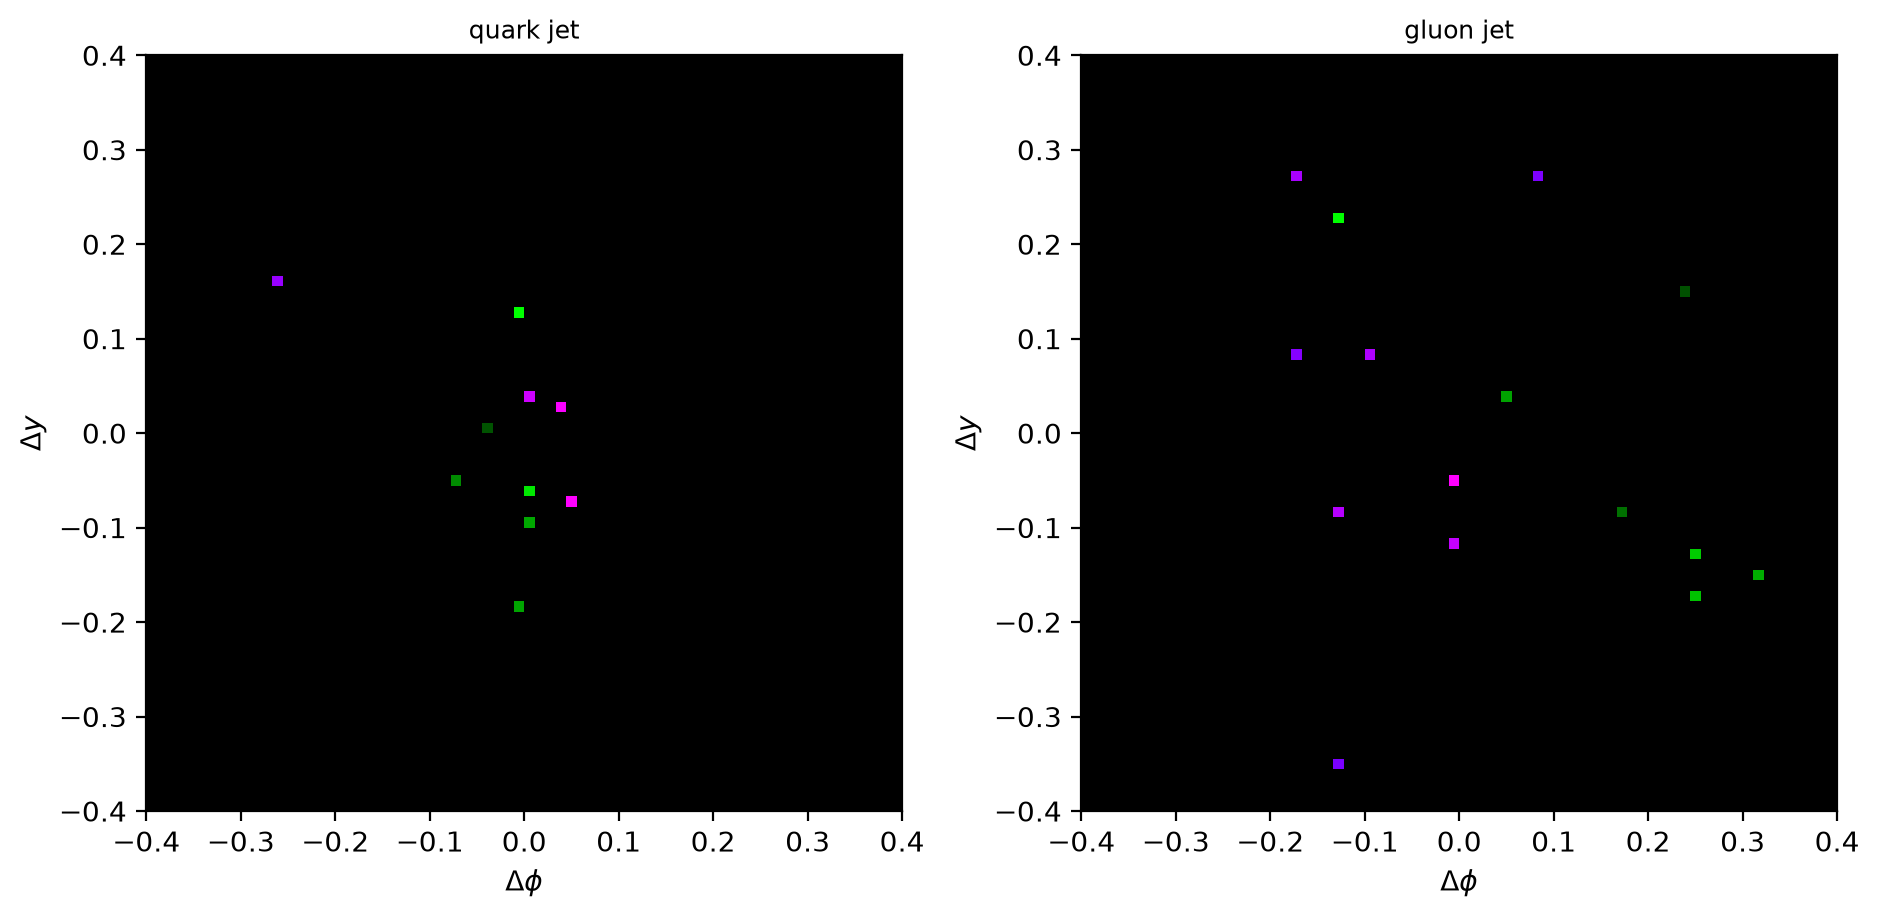
\includegraphics[width=\linewidth]{figures/qgjet_images}
	\caption{Jet images of a typical quark (left) and gluon (right) jet in \(\Delta y\) and \(\Delta\phi\) around the jet axis, with the image channels defined in the text. Gluon jets exhibit a broader spatial radiation pattern
		and higher particle multiplicity compared to quark jets}
	\label{fig:qgJetExamples}
\end{figure}

The images were input for a Convolutional Neural Network (CNN) implemented using PyTorch as shown in fig.~\ref{fig:rgbnn}.  
%
Each convolutional layer consisted of 64 filters, with filter sizes of \(5\times5\), \(3\times3\), and \(3\times3\), respectively. The max-pooling layers performed a 2×2 down-sampling with a stride length of 2. The dense layer consisted of 128 units, with a dropout rate of 0.2 before and after it.
\begin{figure}
	\centering
	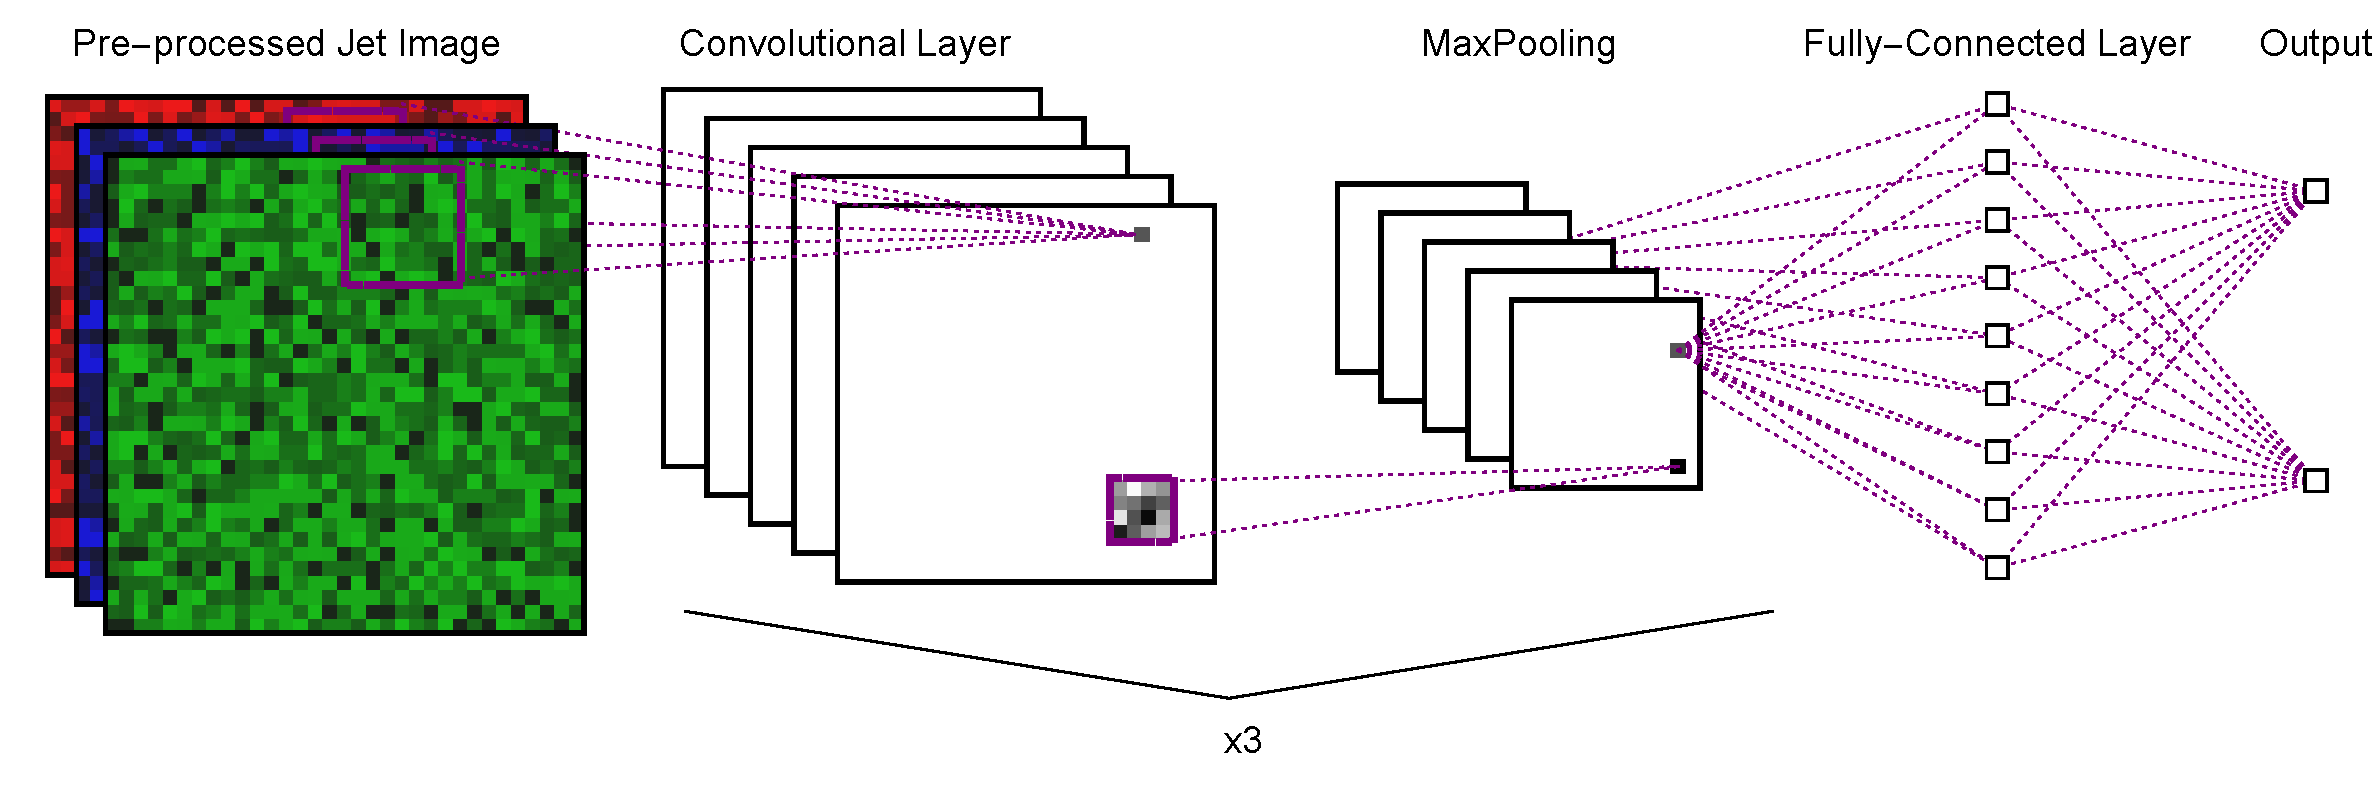
\includegraphics[width=1\linewidth]{figures/RGBNN}
	\caption{An illustration of the deep convolutional neural network architecture. The first
		layer is the input jet image, followed by three convolutional layers, a dense layer and an
		output layer.~\cite{Komiske_2017}}
	\label{fig:rgbnn}
\end{figure}

The network was trained with the AdamW optimizer at a learning rate of \(10^{-3}\) and a weight decay of 0.1, using the cross-entropy loss. 
%
Training used a batch size of 128 for 20 epochs, and the model with the lowest validation loss was retained. 
%
\begin{figure}
	\centering
	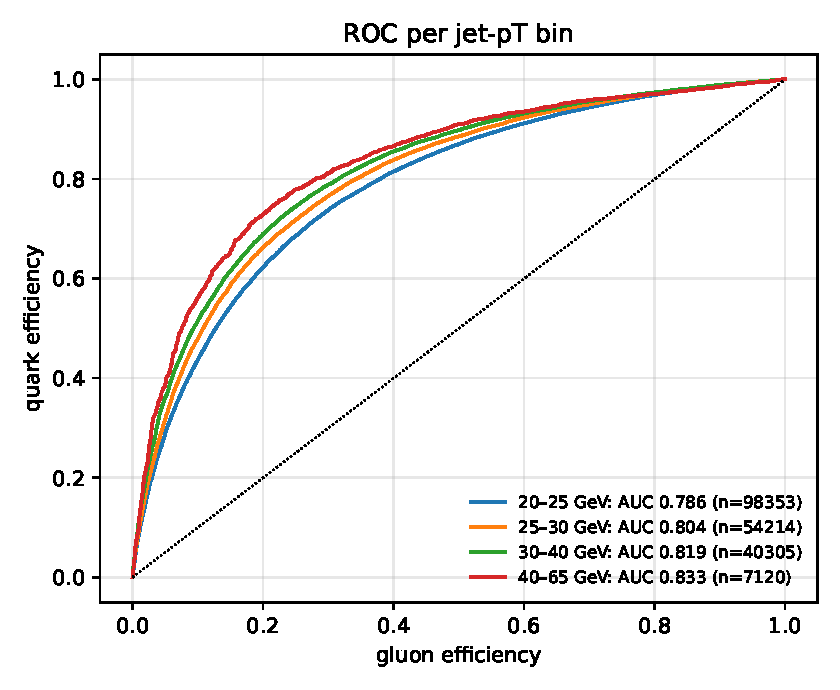
\includegraphics[width=0.7\linewidth]{figures/roc_per_jpt}
	\caption{ROC curves of the CNN quark-gluon classifier, quark efficiency vs gluon efficiency, evaluated on a holdout test set in bins of \(p_\mathrm{T, jet}\) (20--25, 25--30, 30--40 and 40--65 GeV/\(c\)). The area under the curve (AUC) rises from 0.79 to 0.83 with increasing \(p_\mathrm{T, jet}\). The diagonal corresponds to random guessing.}
	\label{fig:rocperjpt}
\end{figure}
Training images were augmented with random reflections in \(\Delta\eta\) and \(\Delta\phi\) and random translations of up to 0.5 pixels. 
%
The Receiver Operator Characteristic (ROC) curve, evaluated on a holdout test set, is shown differentially in \(p_\mathrm{T, jet}\) in Fig.~\ref{fig:rocperjpt}. The separation improves with \(p_\mathrm{T, jet}\), with the area under the curve increasing from 0.79 to 0.83. 


A way to gain some understanding of how the model looks at jet substructure is through \emph{interpretability} methods. 
%
We use a simple method of just noting the average change in classifier output upon masking a pixel. As seen in Fig.~\ref{fig:importancecnnqg}, the classifier relies mostly on the pixels close to the jet axis, and the region it uses becomes narrower for jets with higher \(p_\mathrm{T}\), which are more collimated.
\begin{figure}
	\centering
	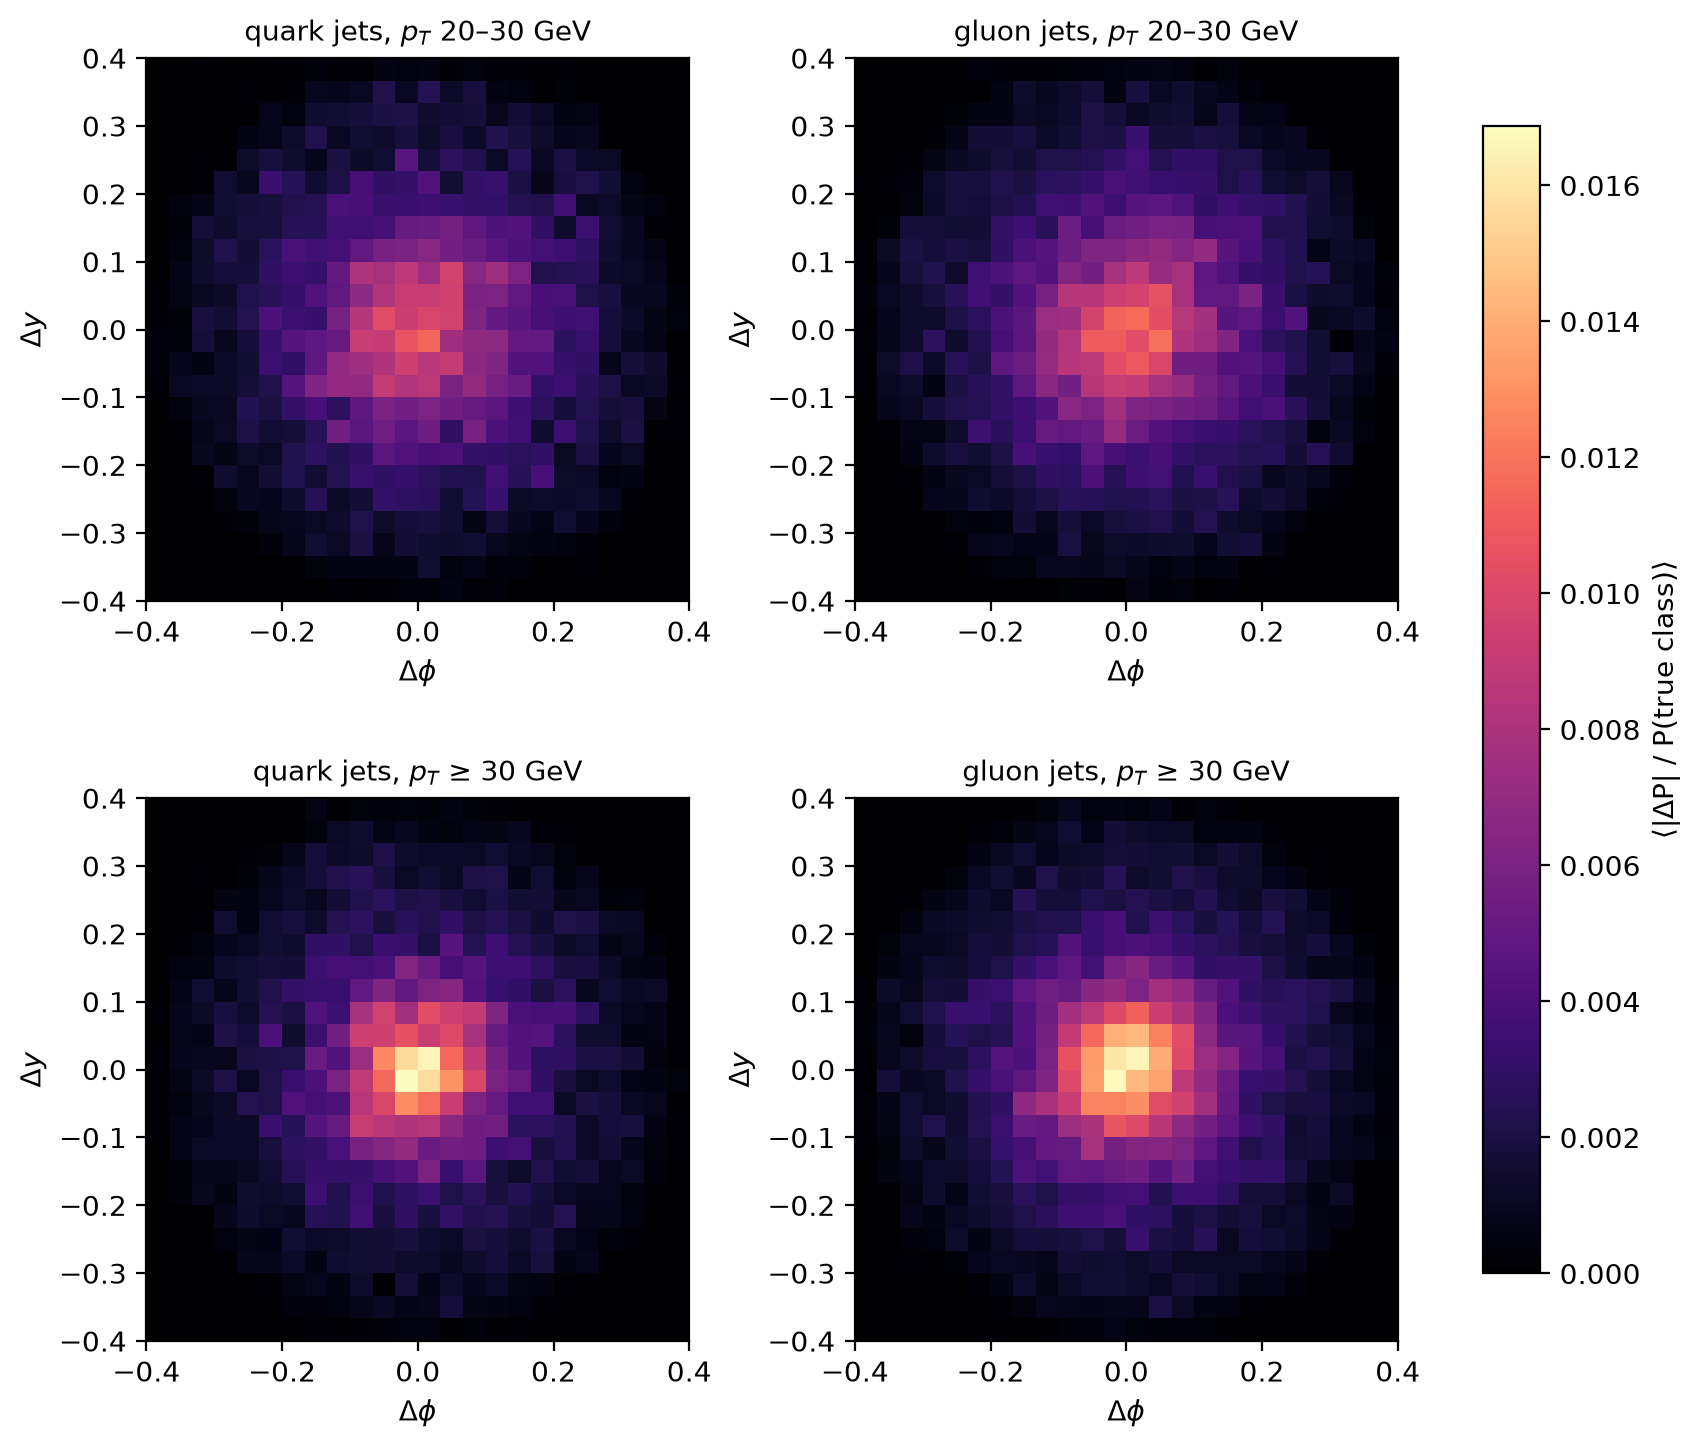
\includegraphics[width=0.7\linewidth]{figures/importance_cnn_qg}
	\caption{Per-pixel importance for the CNN quark-gluon classifier: the mean change of the classifier output when a pixel is masked, relative to the probability of the true class, \(\langle|\Delta P|\rangle/P(\text{true class})\), as a function of \(\Delta y\) and \(\Delta\phi\) from the jet axis, for quark (left) and gluon (right) jets with \(20 < p_\mathrm{T, jet} < 30\)~GeV/\(c\) (top) and \(p_\mathrm{T, jet} \geq 30\)~GeV/\(c\) (bottom).}
	\label{fig:importancecnnqg}
\end{figure}
\subsection{Characterizing jet quenching}
Another way to think about jet quenching/modification, is to ask how easily can a classifier algorithm tell apart the quenched and unquenched jet. 
%
Here we take PYTHIA-6~\cite{Sj_strand_2006} as the source of unquenched jets and JEWEL \cite{Zapp:2013vla} generates quenched jets in different centrality bins with/without recoil centers. 
%
Jets are represented as a 9-D vectors of features: $p_{\rm T, jet}$, $\rm N^{charged}_{\rm constit., jet}$, $\rm N^{neutral}_{\rm constit., jet}$, LeSub, $\lambda^2_0$, $\lambda_1^{0.5}$, $\lambda_1^1$, $\lambda_1^2$.
%
The jets are input into Dense Neural Networks (DNNs) with three hidden layers with 100 nodes each. After training, we calculate ROC curves shown in Fig.~\ref{fig:jetQuenchROC} using a holdout test set.
%
\begin{figure}
	\includegraphics[width=0.49\linewidth]{roc_curve_dnn_withoutRec.pdf}
	\includegraphics[width=0.49\linewidth]{roc_curve_dnn_wRec.pdf}
	\caption{ROC curves of the DNN classifier separating PYTHIA-6 (unquenched) from JEWEL (quenched) jets, for JEWEL without recoils (left) and with recoils (right), in four centrality classes, with the corresponding AUC values in the legends. Jets are anti-\(k_\mathrm{T}\), \(R = 0.4\), \(p_\mathrm{T, jet} > 10\)~GeV/\(c\), \(|\eta_\mathrm{jet}| < 1 - R\), with at least two charged constituents.}
	\label{fig:jetQuenchROC}
\end{figure}
%
The DNN performs better than chance in all the centralities and for both with/without recoils case.
The with-recoils case gives exagerrated ROC curves due to the background of recoil centers. 
%
AUC score decreases from central (0-10\%) to peripheral (50-80\%) events possibly implying more modification in central compared to peripheral.  
%
More information about jet quenching and machine learning can be found in~\cite{lai2022informationcontentjetquenching}
